\documentclass[12pt]{article}
\usepackage[T1]{fontenc}
\usepackage[utf8]{inputenc}
\usepackage{textcomp}
\usepackage[english,french]{babel}
\usepackage{etex}
\usepackage[left=0.5in, right=0.5in, top=1.0in, bottom=1.0in]{geometry}
\usepackage{layout}
\usepackage{lmodern}
\usepackage{stmaryrd}
\usepackage{amsthm}
\usepackage{amsmath}
\usepackage{amsfonts}
\usepackage{amssymb}
\usepackage{textcomp}
\usepackage{graphicx}
\usepackage{hyperref}
\usepackage[all]{hypcap}
\usepackage{tabularx}
\usepackage[usenames,dvipsnames]{xcolor}
\usepackage{listings}
\usepackage{algorithm2e}
\usepackage{verbatim}
\hypersetup{
  bookmarks=true,         % show bookmarks bar?
  unicode=false,          % non-Latin characters in Acrobat’s bookmarks
  pdftoolbar=true,        % show Acrobat’s toolbar?
  pdfmenubar=true,        % show Acrobat’s menu?
  pdffitwindow=false,     % window fit to page when opened
  pdfstartview={FitH},    % fits the width of the page to the window
  pdftitle={My title},    % title
  pdfauthor={Author},     % author
  pdfsubject={Subject},   % subject of the document
  pdfcreator={Creator},   % creator of the document
  pdfproducer={Producer}, % producer of the document
  pdfkeywords={keyword1} {key2} {key3}, % list of keywords
  pdfnewwindow=true,      % links in new window
  colorlinks=true,       % false: boxed links; true: colored links
  linkcolor=cyan,          % color of internal links (change box color with linkbordercolor)
  citecolor=green,        % color of links to bibliography
  filecolor=magenta,      % color of file links
  urlcolor=cyan           % color of external links
}
\usepackage{parcolumns}
\begin{document}


\lstset{                                    % line wrapping on
  language=C,
  frame=lines,
  captionpos=b
 }

\renewcommand{\lstlistingname}{Code}
\section*{APPENDIX}

 The programs used for Odd-Even Merge sort and Bitonic sort are provided below : \\ 

\noindent\begin{minipage}{.45\textwidth}
\begin{lstlisting}[label=bitsort, caption=Bitonic Sort : sort from m to n,frame=tlrb]{Name}
sortup( int m, int n) {
//from m to m+n
    if (n == 1) return;
    sortup(m, n/2);
    sortdown(m + n/2, n/2);
    mergeup(m, n/2);
}
 sortdown(int m, int n) {
//from m to m+n
    if (n == 1) return;
    sortup(m, n/2);
    sortdown(m + n/2, n/2);
    mergedown(m, n/2);
}

\end{lstlisting}
\end{minipage}\hfill
\begin{minipage}{.50\textwidth}
\begin{lstlisting}[label=bitmerge, caption = Bitonic Merge,frame=tlrb]{Name}
mergeup(int m, int n) {  
    if (n == 0) return;
    
    for (i = 0 : n)
        // Increasing Comparator
	 compare(m + i,m + i + n);
    mergeup(m, n/2);
    mergeup(m + n,n/2);
}

mergedown( int m,  int n) { 
    if (n == 0) return;
    for (i = 0 : n) 
        // Decreasing Comparator
	compare(m + i, m + i + n); 
    mergedown(m, n/2);
    mergedown(m + n, n/2);
}
\end{lstlisting}
\end{minipage}
\noindent\begin{minipage}{.45\textwidth}
\begin{lstlisting}[label=oemerge, caption=Odd-Even Merge,frame=tlrb]{Name}
oddEvenMerge(int lo, int n, int r){
  int m = r*2;
  if (m < n){
    //even subsequence ;		
    oddEvenMerge(lo, n, m); 
    //odd subsequence ;
    oddEvenMerge(lo+r, n, m); 
    int i = lo+r;   
    for (;i + r < lo + n;){
      compare(i, i + r);
      i += m;
    }
  }
  else
  compare(lo, lo + r);
}
\end{lstlisting}
\end{minipage}\hfill
\begin{minipage}{.50\textwidth}
\begin{lstlisting}[label=oesort, caption = Odd-Even sort from lo to n,frame=tlrb]{Name}

 OddEvenMergeSort(int lo, int n)
if (n > 1){
  int m = n/2;
  oddEvenMergeSort(lo, m);
  oddEvenMergeSort(lo + m, m);
  oddEvenMerge(lo, n, 1);
}
\end{lstlisting}
\end{minipage}


\begin{figure}
\centering
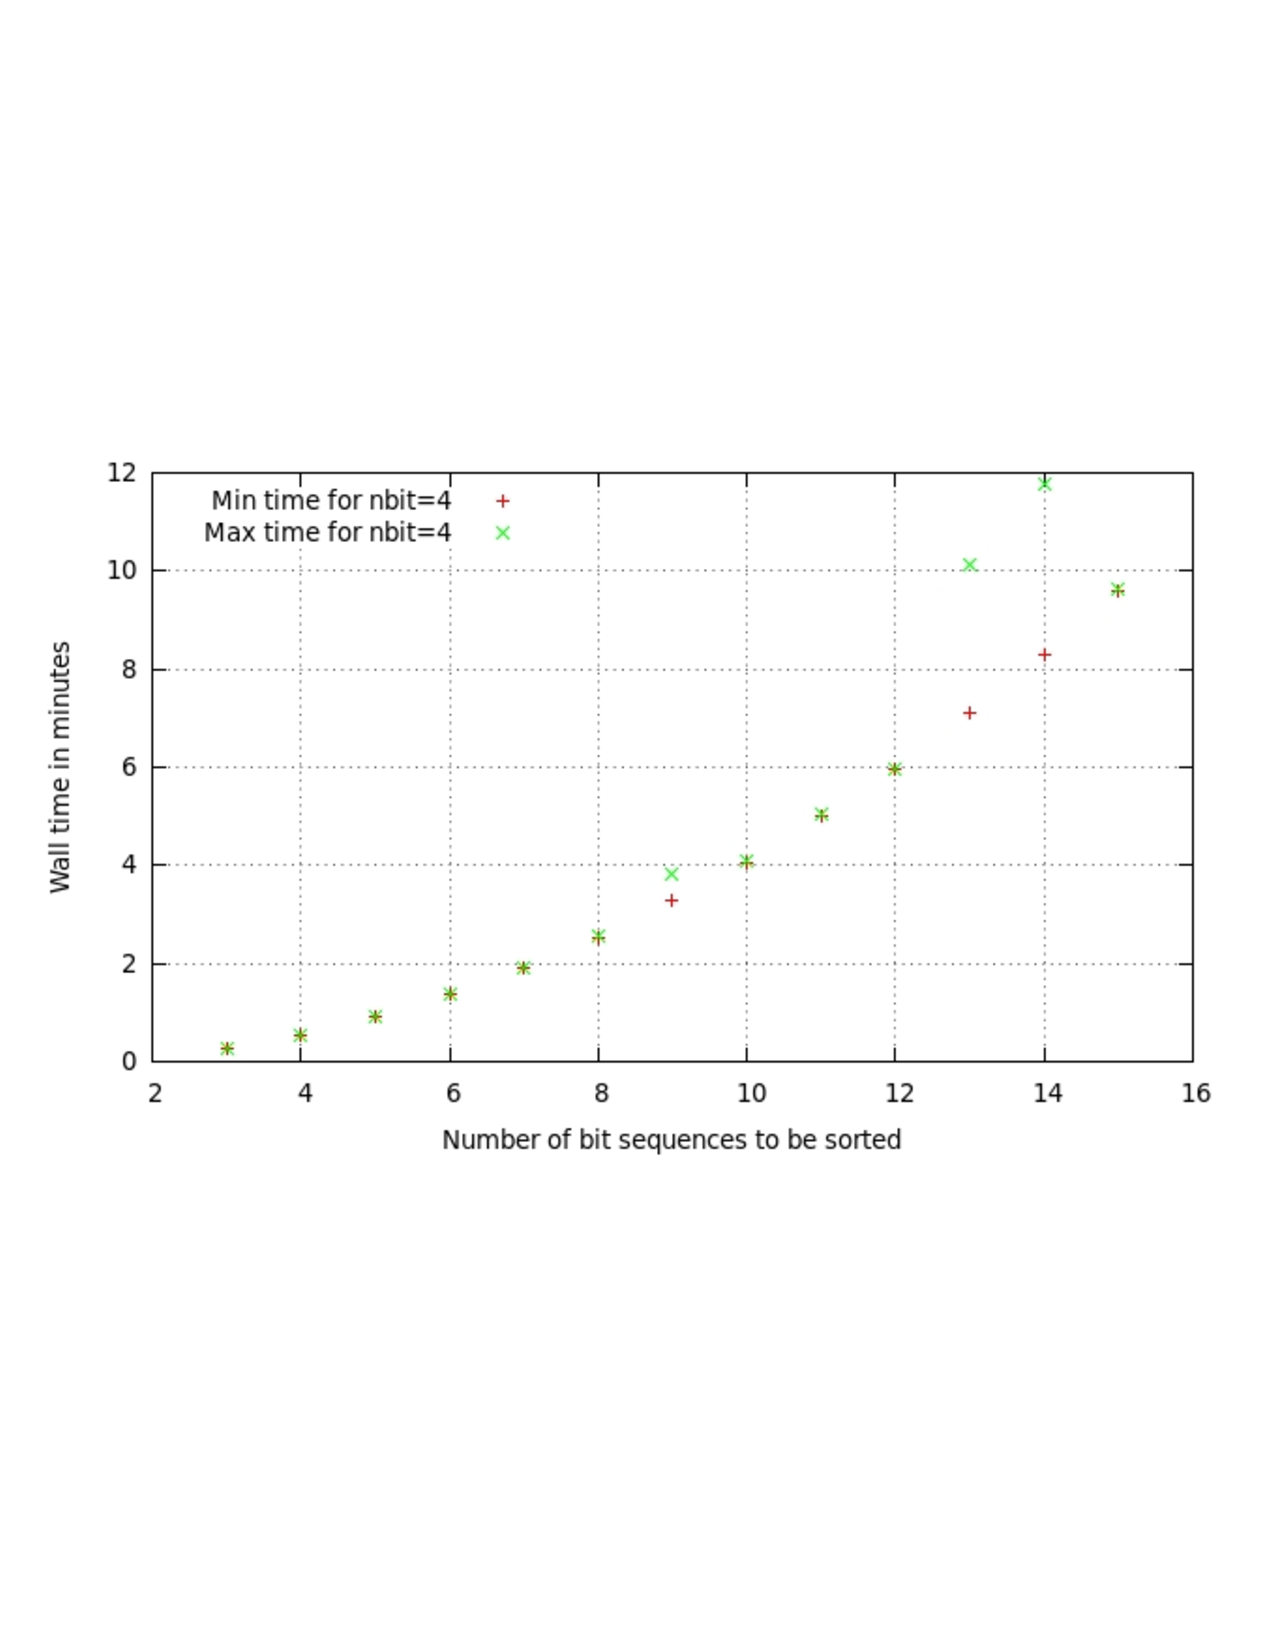
\includegraphics[width=12cm]{fsort3.pdf} 
\caption{Run time for Insertion sort, nbit=4} 
\label{fig:image_sf3} %l'étiquette pour faire référence à cette image
\end{figure}

\begin{figure} %on ouvre l'environnement figure
\centering
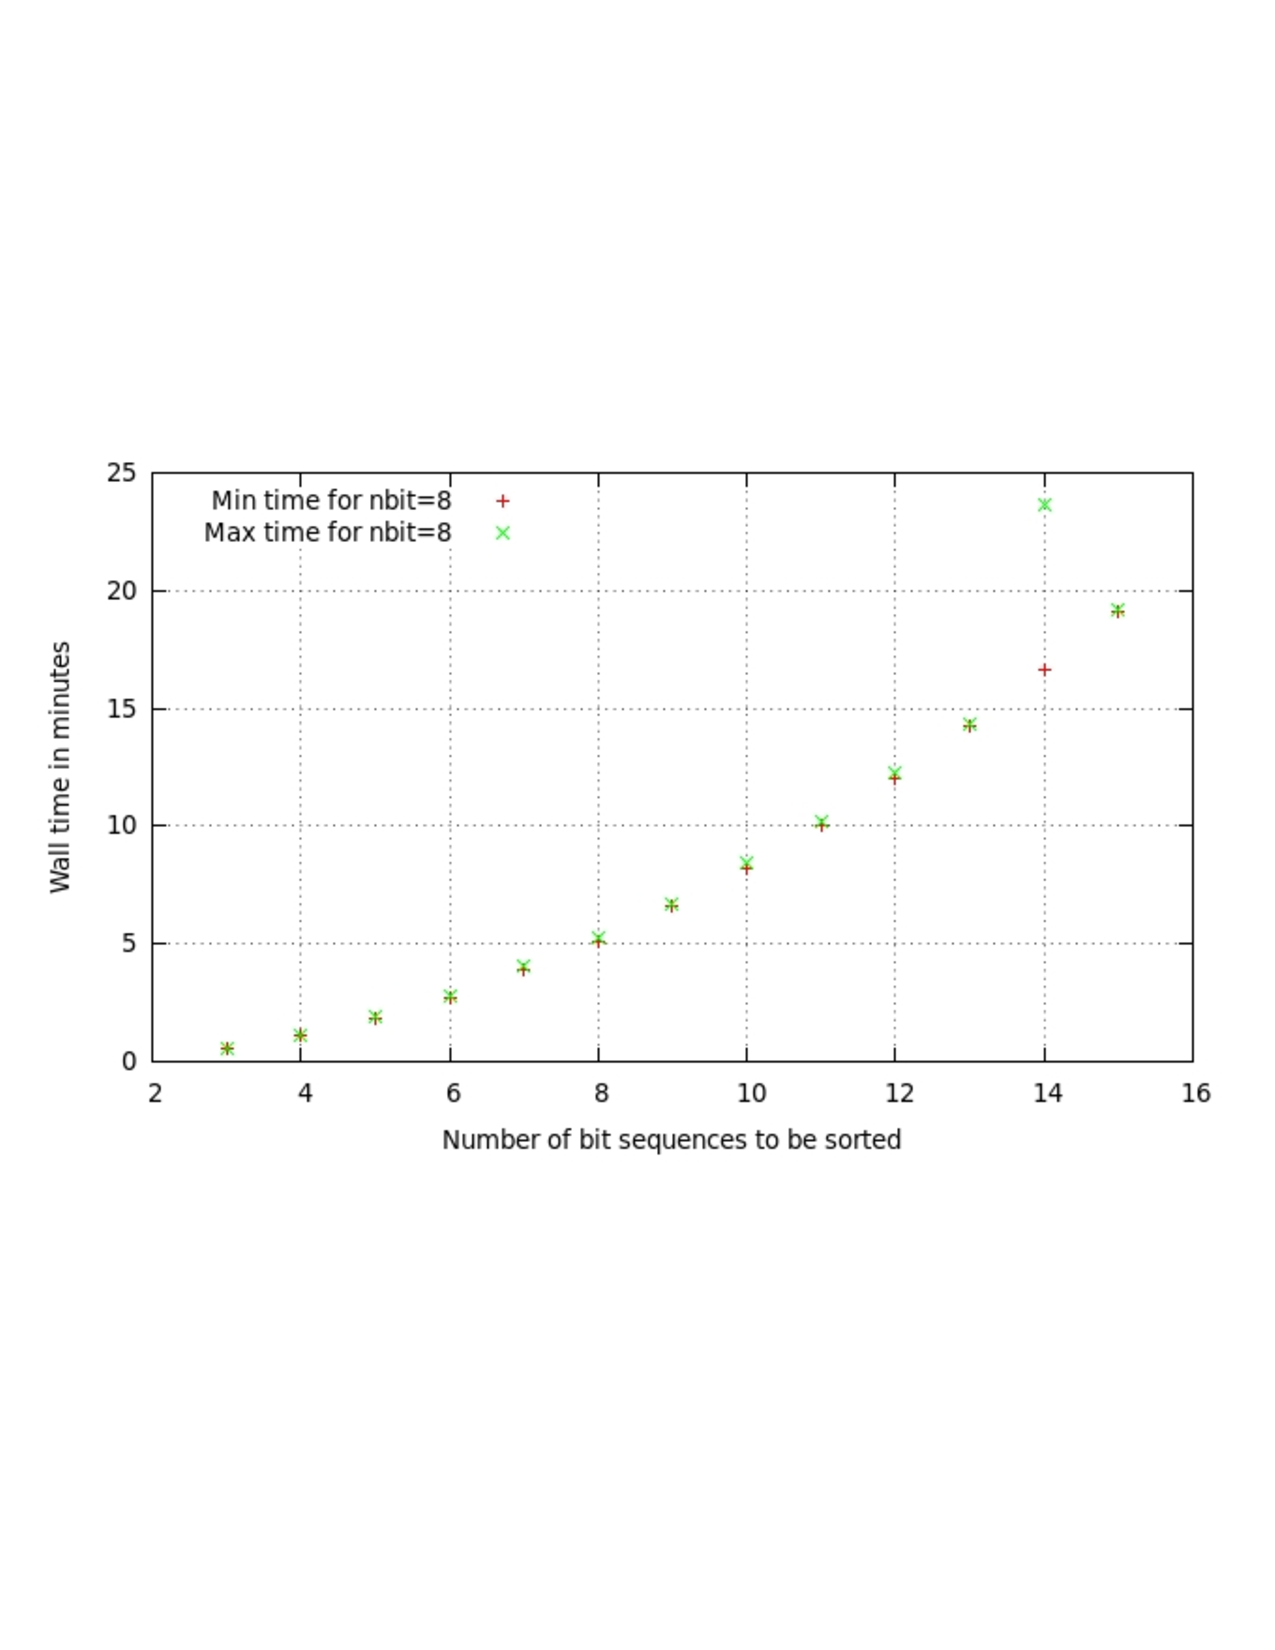
\includegraphics[width=12cm]{fsort5.pdf} 
\caption{Run time for Insertion sort, nbit=8} 
\label{fig:image_sf5} %l'étiquette pour faire référence à cette image
\end{figure}


\begin{figure}%on ouvre l'environnement figure
\centering
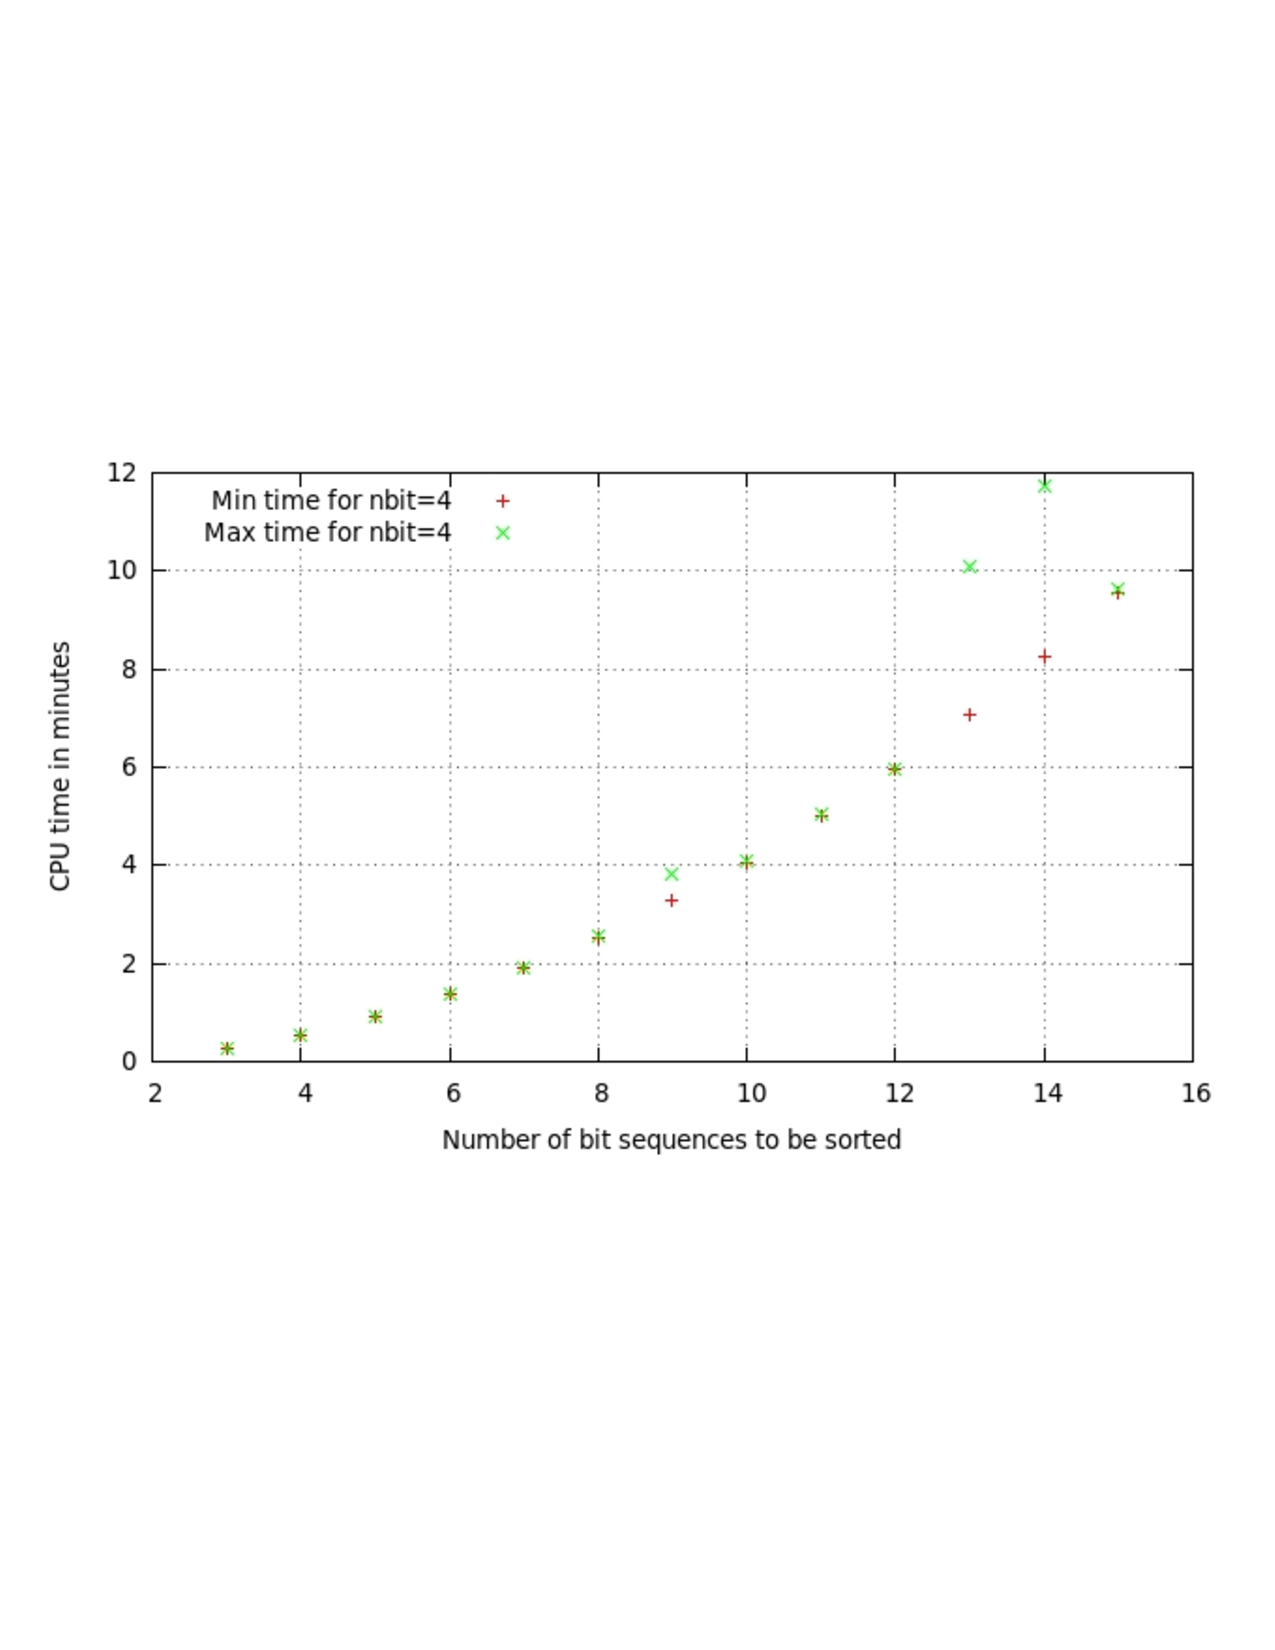
\includegraphics[width=12cm]{fsort6.pdf} 
\caption{CPU time for Insertion sort, nbit=4} 
\label{fig:image_sf6} %l'étiquette pour faire référence à cette image
\end{figure}

\begin{figure}%on ouvre l'environnement figure
\centering
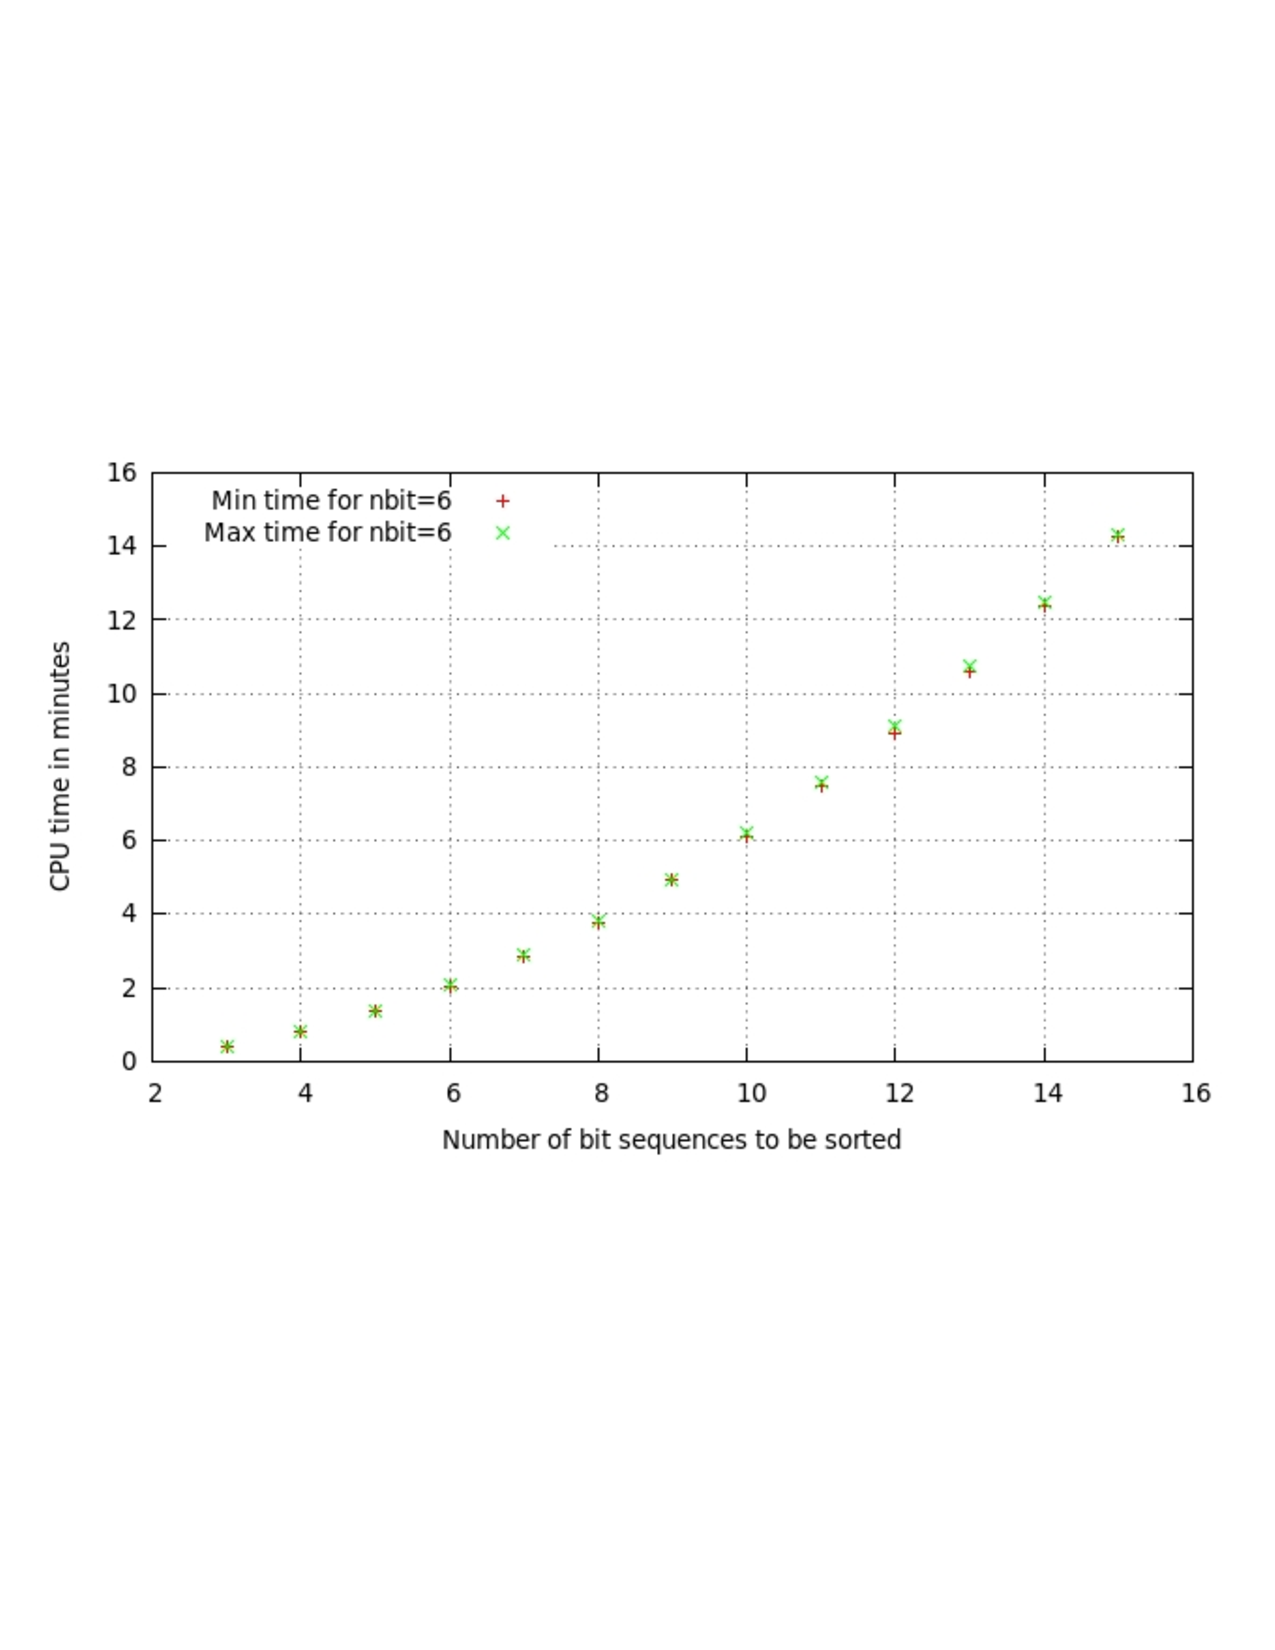
\includegraphics[width=12cm]{fsort8.pdf} 
\caption{CPU time for Insertion sort, nbit=6} 
\label{fig:image_sf8} %l'étiquette pour faire référence à cette image
\end{figure}


\begin{figure}%on ouvre l'environnement figure
\centering
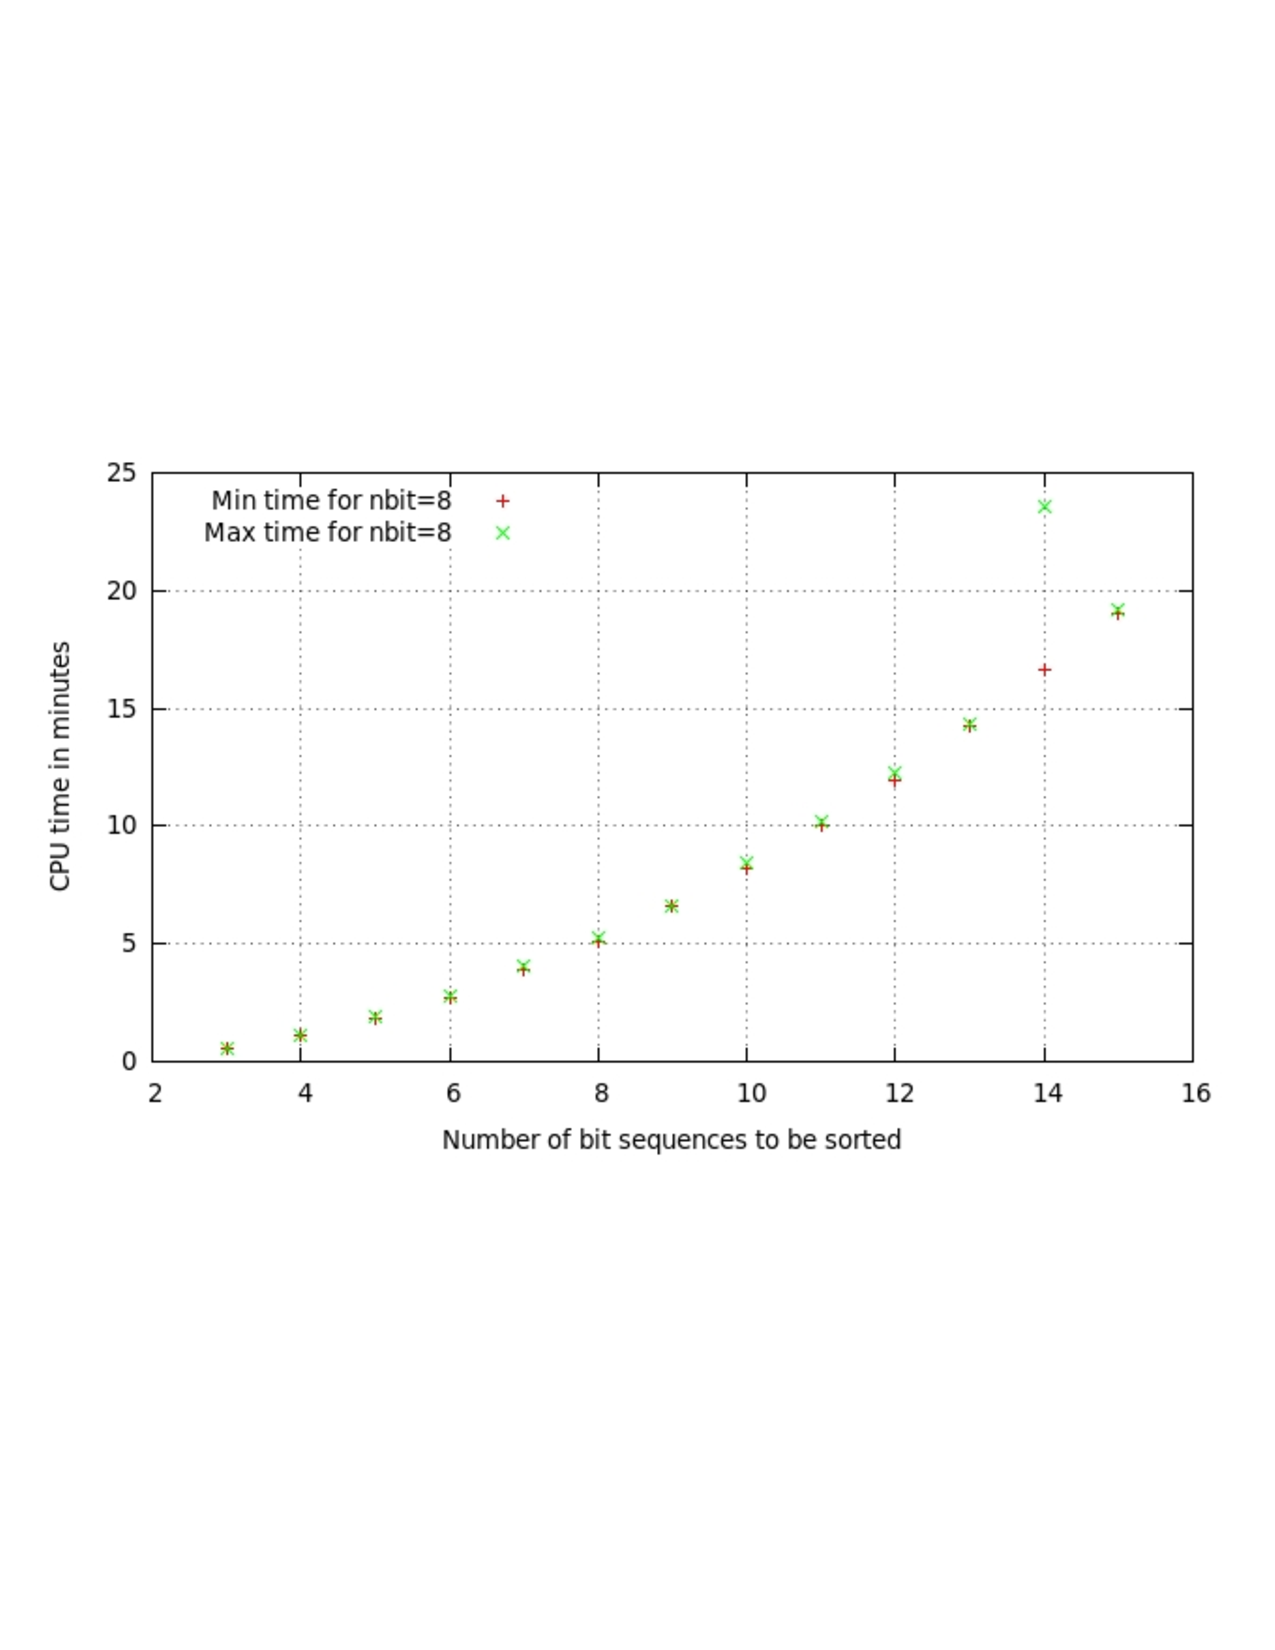
\includegraphics[width=12cm]{fsort7.pdf} 
\caption{CPU time for Insertion sort, nbit=8} 
\label{fig:image_sf7} %l'étiquette pour faire référence à cette image
\end{figure}

\end{document}
